\section*{CHƯƠNG 4 - QUY TRÌNH TỰ ĐỘNG HÓA}
\addcontentsline{toc}{section}{\numberline{}CHƯƠNG 4 -  QUY TRÌNH TỰ ĐỘNG HÓA}
\setcounter{section}{4}
\setcounter{subsection}{0}
\setcounter{figure}{0}
\setcounter{table}{0}

%-----------Phần trình bày nội dung chương 4

\subsection{Tổng quan hệ thống}
    Hệ thống tự động hóa cấu hình mạng (Network Automation System) được viết bằng Python, sử dụng thư viện Netmiko để quản lý và cấu hình các thiết bị mạng Cisco (Router và Switch). Hệ thống này cho phép tự động hóa việc cấu hình, giám sát, backup và restore cấu hình cho nhiều thiết bị mạng cùng lúc, giúp tiết kiệm thời gian và giảm thiểu sai sót so với cấu hình thủ công. 
    Các chức năng chính:
    
    \begin{itemize}
        \item Cấu hình VLAN cho Switch
        \item Cấu hình IP Interface cho Router
        \item Cấu hình OSPF routing
        \item Cấu hình Static Route
        \item Backup và Restore cấu hình
        \item Giám sát thiết bị mạng
    \end{itemize}
\subsection{Thiết lập hệ thống GNS3-VM}
\subsubsection{Yêu cầu hệ thống}
    \begin{itemize}
    \item[*] Phần cứng:
    \item CPU: Intel Core i5/i7 hỗ trợ VT-x/AMD-V
    \item RAM: 8GB (tối thiểu), 16GB (khuyến nghị)
    \item Ổ cứng: 50GB
    \item[*] Phần mềm:
    \item GNS3 GUI 2.2.46+
    \item GNS3-VM 2.2.46+
    \item VMware Workstation 17
    \item Kiểm tra VT-x: Task Manager → Performance → CPU →Virtualization.
    \item Enabled
    \end{itemize}
\subsubsection{Các bước cài đặt}
    \begin{itemize}
    \item Cài đặt GNS3-VM để hỗ trợ môi trường mô phỏng.
    \item Cài GNS3 GUI để thao tác và quản lý mô hình.
    \item Import IOS để sử dụng thiết bị Cisco trong dự án.
    \item Thiết lập kết nối mạng giữa các thành phần.
    \item Cấu hình NAT cho phép thiết bị truy cập Internet.
    \item Bật SSH để điều khiển từ xa qua script.
    \item Tạo file devices.csv lưu danh sách thiết bị.
    \item Kiểm thử quá trình tự động hóa bằng Python.
    \end{itemize}

\subsection{Kiến trúc tổng thể hệ thống tự động hoá}

    Sơ đồ kiến trúc:
        \begin{figure}[H]
            \centering
            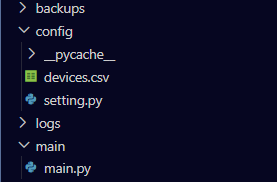
\includegraphics[width=0.7\textwidth]{image/cau_truc_code_1.png}
        \end{figure}
    
        \begin{figure}[H]
            \centering
            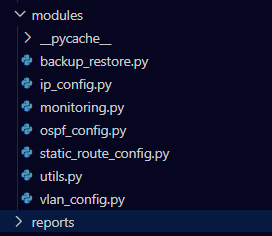
\includegraphics[width=0.7\textwidth]{image/cau_truc_code_2.png}
            \caption{Cấu trúc tổng quan}
        \end{figure}
 
\subsection{Phân tích chi tiết từng file}
\subsubsection{setting.py - File cấu hình toàn cục}
    Mục đích:
    \begin{itemize}
        \item Lưu trữ tất cả cấu hình mạng và thiết lập đường dẫn
    \end{itemize}
    Nội dung:
    \begin{itemize}
        \item Đường dẫn: BASE\_DIR, REPORTS\_DIR, LOGS\_DIR, BACKUPS\_DIR, CONFIG\_DIR.
        \item Tham số kết nối: CONNECTION\_TIMEOUT, DEVICE\_DELAY.
        \item VLAN\_CONFIGS: Cấu hình VLAN cho 3 Switch (VLAN 10, 20, 99; trunk và access ports).
        \item IP\_CONFIGS: Cấu hình IP cho 3 Router (interface, subinterface với encapsulation dot1q).
        \item OSPF\_CONFIGS: Cấu hình OSPF routing cho 3 Router (process 1, area 0).
        \item STATIC\_ROUTE\_CONFIGS: Cấu hình static route cho 3 Router.
        \item create\_directories(): Tạo các thư mục cần thiết.
    \end{itemize}
\subsubsection{utils.py - Module tiện ích chung}

    Mục đích: Cung cấp các hàm tiện ích được sử dụng chung.
    Các hàm chính:
    
    \begin{itemize}
        \item setup\_logging(): Thiết lập logging (ghi log ra file và console).
        \item load\_devices(): Đọc danh sách thiết bị từ file CSV.
        \item get\_device\_info(): Chuyển đổi thông tin thiết bị sang định dạng dict cho Netmiko.
        \item save\_results(): Lưu kết quả ra file CSV với timestamp.
        \item print\_header(): In header với tiêu đề và thời gian.
        \item print\_summary(): In tổng kết (thành công/thất bại).
        \item filter\_devices(): Lọc thiết bị theo loại hoặc hostname.
        \item confirm\_action(): Yêu cầu xác nhận từ người dùng.
        \item display\_menu(): Hiển thị menu và nhận input.
    \end{itemize}
        
\subsubsection{vlan\_config.py - Module cấu hình VLAN}
    Mục đích: Tự động cấu hình VLAN trên Switch.
    Các hàm chính:
    \begin{itemize}
        \item configure\_vlan(): Cấu hình VLAN cho một Switch.
            \begin{figure}[H]
                \centering
                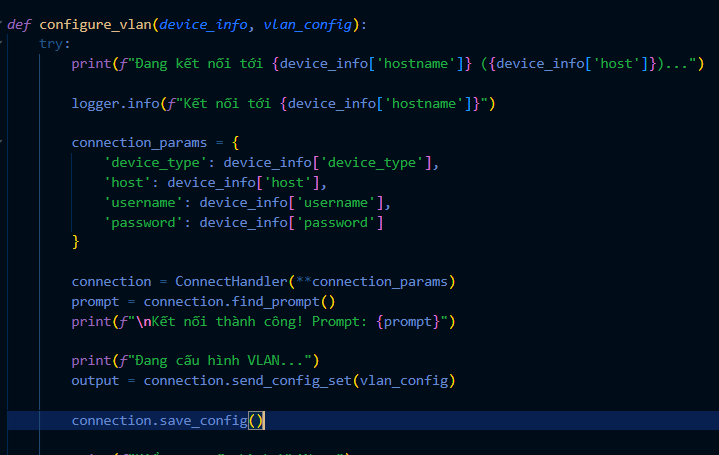
\includegraphics[width=0.7\textwidth]{image/configure_vlan_1.png}
            \end{figure}

            \begin{figure}[H]
                \centering
                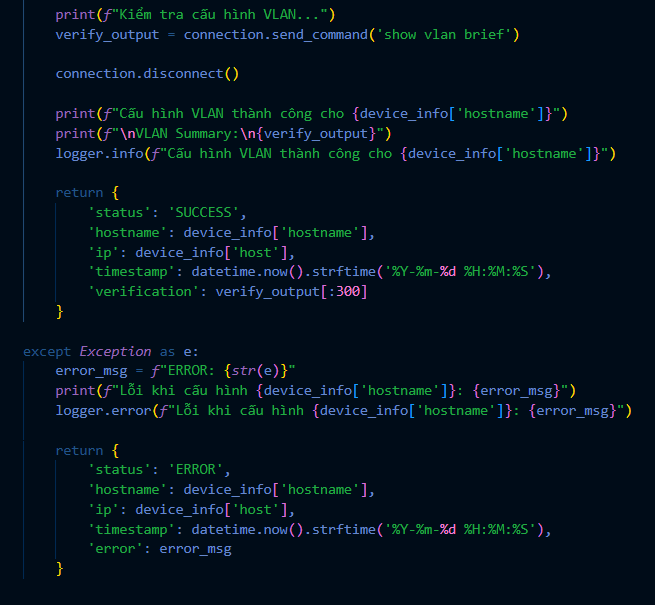
\includegraphics[width=0.7\textwidth]{image/configure_vlan_2.png}
                \caption{Cấu hình VLAN cho một Switch}
            \end{figure}
            
            
        \item configure\_all\_vlans(): Cấu hình VLAN cho tất cả Switch.
            \begin{figure}[H]
                \centering
                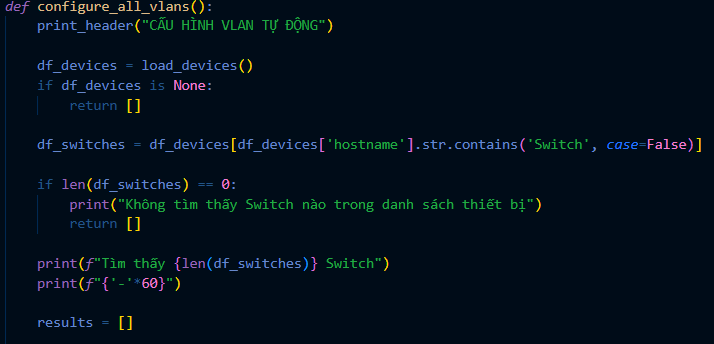
\includegraphics[width=0.7\textwidth]{image/cf_a_vlan_1.png}
            \end{figure}

            \begin{figure}[H]
                \centering
                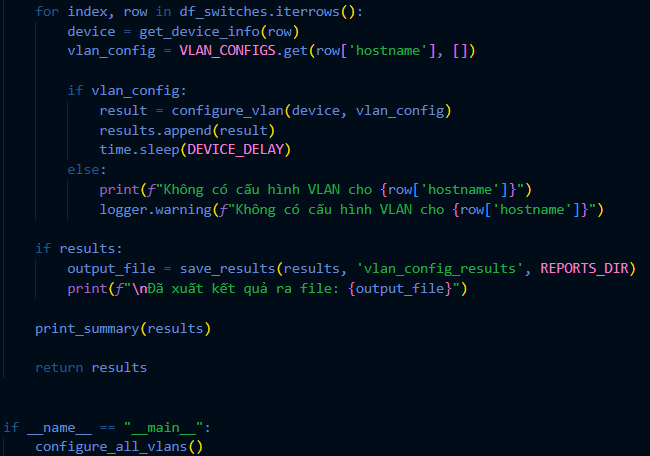
\includegraphics[width=0.7\textwidth]{image/cf_a_vlan_2.png}
                \caption{Cấu hình VLAN cho tất cả Switch}
            \end{figure}         
    \end{itemize}    
    
    \_Ý nghĩa: 
    \begin{itemize}
        \item Tạo VLAN.
        \item Cấu hình trunk port và access port.
        \item Verify bằng show vlan brief.
    \end{itemize}
\subsubsection{ip\_config.py - Module cấu hình IP Interface}
    Mục đích:Tự động cấu hình địa chỉ IP cho các interface trên Router.
    Các hàm chính:
    \begin{itemize}
        \item  configure\_ip\_interface():Cấu hình IP cho một Router.
            \begin{figure}[H]
                \centering
                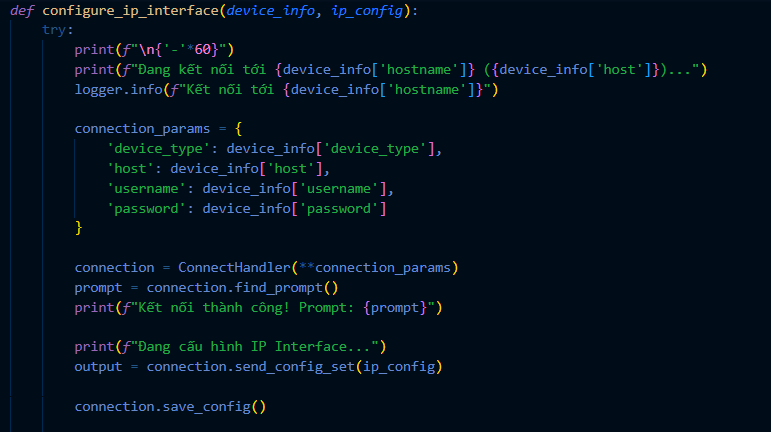
\includegraphics[width=0.7\textwidth]{image/cf_ip_if_1.png}
            \end{figure}

            \begin{figure}[H]
                \centering
                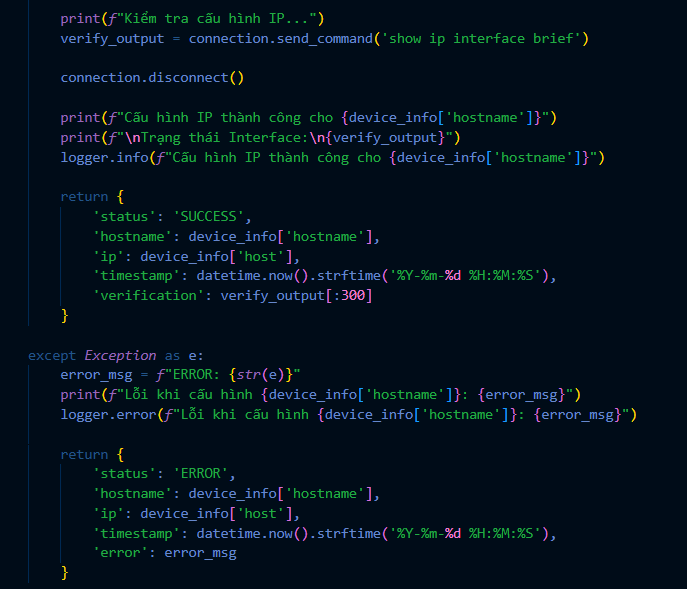
\includegraphics[width=0.7\textwidth]{image/cf_ip_if_2.png}
                \caption{Cấu hình IP cho interface trên Router}
            \end{figure}

            
        \item configure\_all\_ip\_interfaces():Áp dụng cấu hình IP cho tất cả Router.
            \begin{figure}[H]
                \centering
                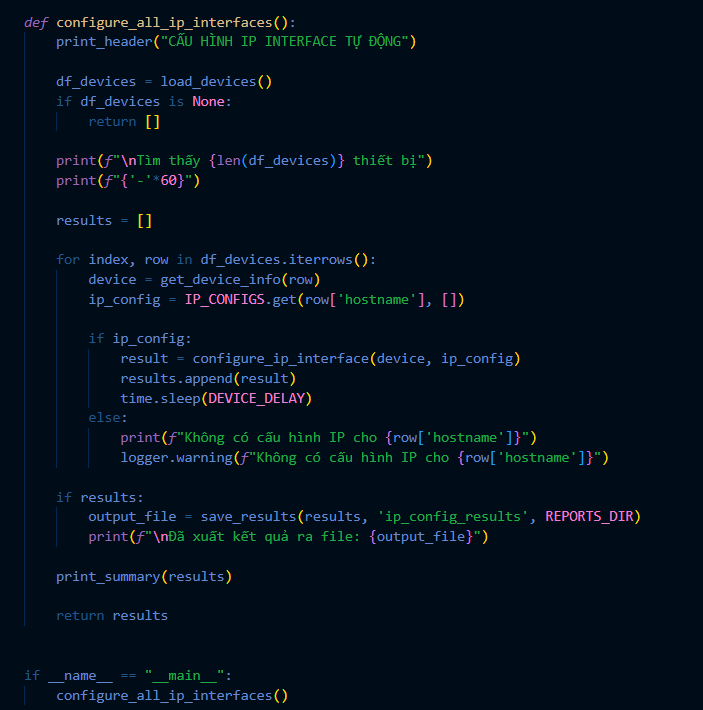
\includegraphics[width=0.5\textwidth]{image/cf_a_ip_if.png}
                \caption{Cấu hình IP cho tất cả interface trên Router}
            \end{figure}
    \end{itemize}

    \_Ý nghĩa:
    \begin{itemize}
        \item  Kết nối đến Router.
        \item  Gửi danh sách lệnh cấu hình IP.
        \item  Lưu cấu hình (write memory).
        \item  Verify bằng lệnh show ip interface brief.
    \end{itemize}
        
\subsubsection{ospf\_config.py - Module cấu hình OSPF}
    Mục đích: Tự động cấu hình giao thức định tuyến OSPF
    Các hàm chính:
    \begin{itemize}
        \item configure\_ospf(): Cấu hình OSPF cho một Router.
            \begin{figure}[H]
                \centering
                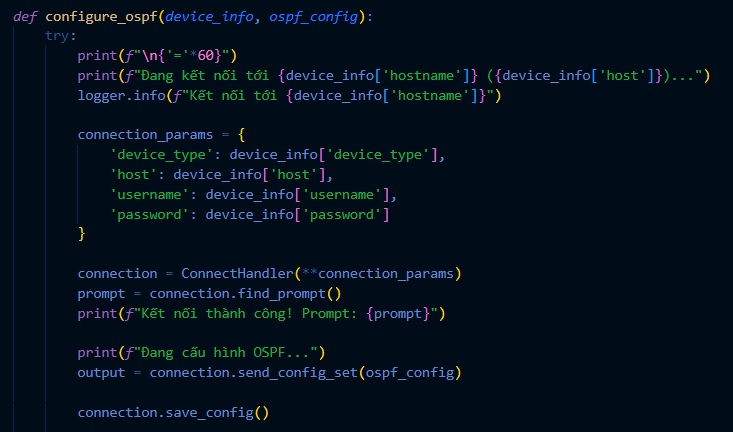
\includegraphics[width=0.7\textwidth]{image/cf_ospf_1.png}
            \end{figure}

            \begin{figure}[H]
                \centering
                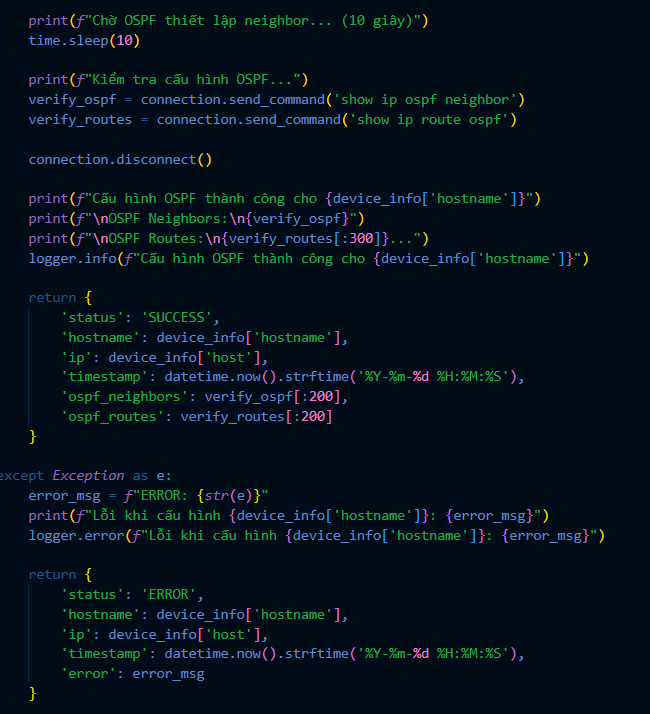
\includegraphics[width=0.7\textwidth]{image/cf_ospf_2.png}
                \caption{Cấu hình IP cho tất cả interface trên Router}
            \end{figure}

        \item configure\_all\_ospf(): Cấu hình OSPF cho tất cả Router.
            \begin{figure}[H]
                \centering
                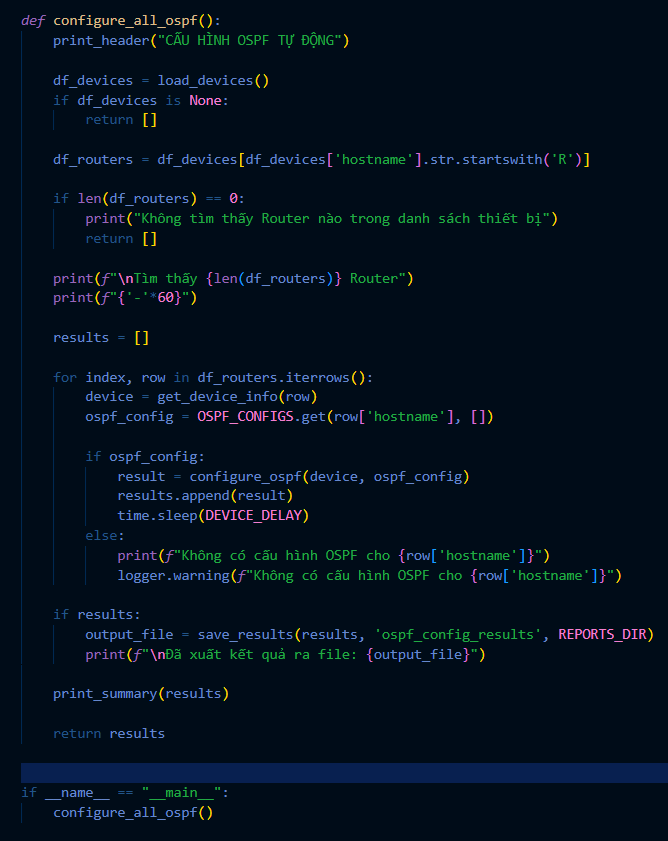
\includegraphics[width=0.7\textwidth]{image/cf_a_ospf.png}
                \caption{Cấu hình IP cho tất cả interface trên Router}
            \end{figure}
    \end{itemize}
    \_Ý nghĩa:
    \begin{itemize}
        \item Áp dụng cấu hình OSPF (router-id, network statements)
        \item Chờ 10 giây để OSPF neighbor thiết lập
        \item Verify bằng show ip ospf neighbor và show ip route ospf
    \end{itemize}
    

\subsubsection{static\_route\_config.py - Module cấu hình Static Route}
    Mục đích:Tự động cấu hình static route (thay thế OSPF nếu cần).
    Các hàm chính:
    \begin{itemize}
        \item configure\_static\_route():Cấu hình static route cho một Router.
        \begin{figure}[H]
                \centering
                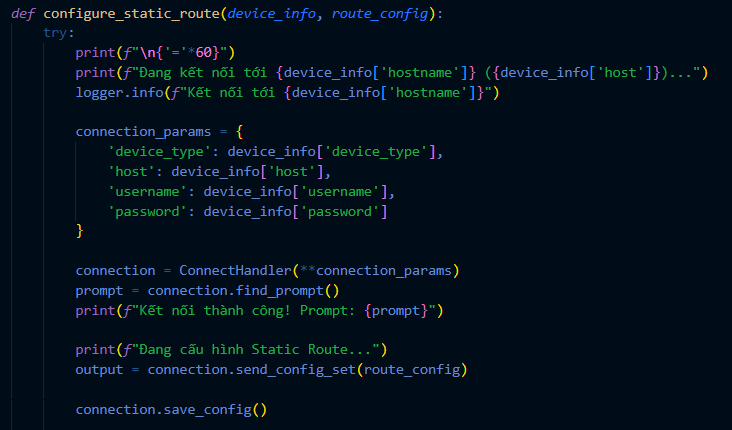
\includegraphics[width=0.7\textwidth]{image/cf_st_1.png}
                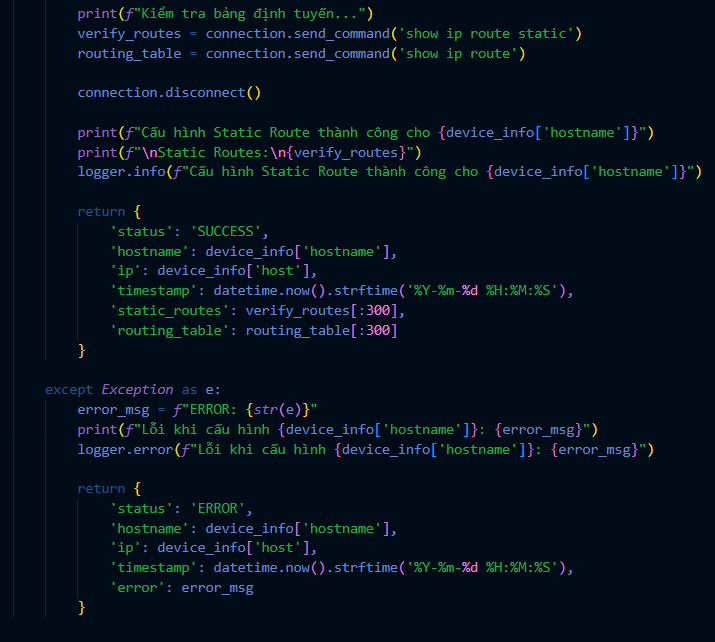
\includegraphics[width=0.7\textwidth]{image/cf_st_2.png}
                \caption{Cấu hình định tuyến tĩnh cho một Router}
        \end{figure}
        
        \item configure\_all\_static\_routes():  Cấu hình static route cho tất cả Router.
        \begin{figure}[H]
                \centering
                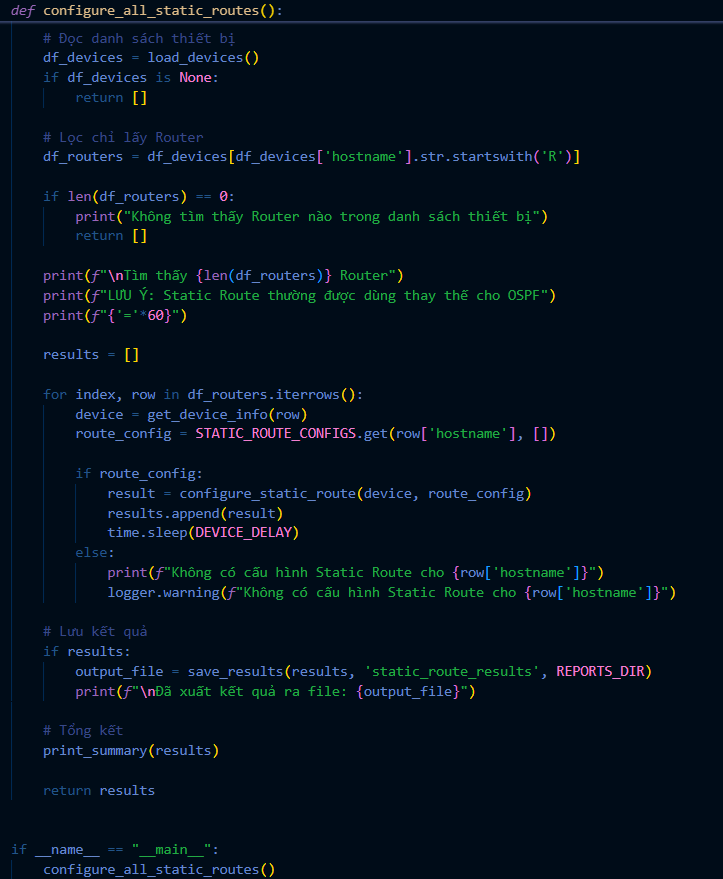
\includegraphics[width=0.7\textwidth]{image/cf_a_st.png}
                \caption{Cấu hình định tuyến tĩnh cho tất cả Router}
        \end{figure}
        
    \end{itemize}
    \_Ý nghĩa:
    \begin{itemize}
        \item Áp dụng các lệnh ip route.
        \item Verify bằng show ip route static.
    \end{itemize}


\subsubsection{backup\_restore.py - Module Backup \& Restore}
    Mục đích:Quản lý backup và khôi phục cấu hình thiết bị
    Các hàm chính:
    \begin{itemize}
        \item backup\_config():Backup cấu hình một thiết bị (lấy running-config).
        \begin{figure}[H]
                \centering
                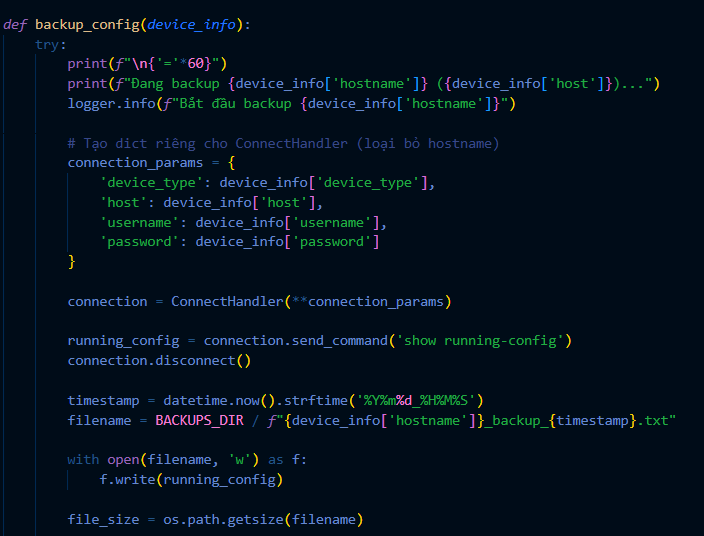
\includegraphics[width=0.7\textwidth]{image/bu_cf_1.png}
                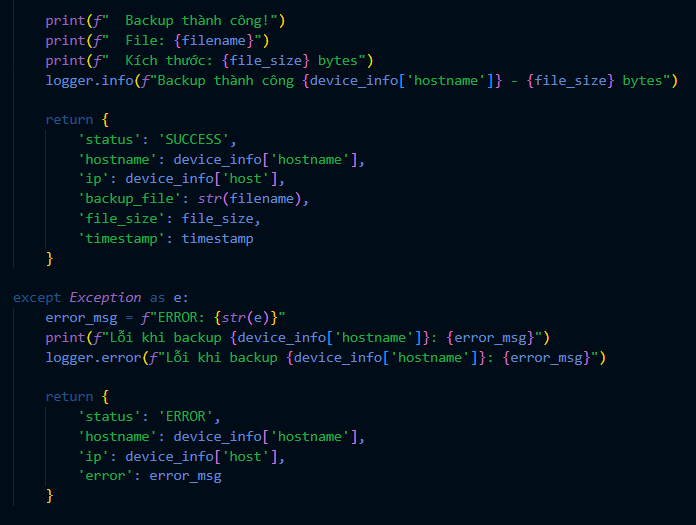
\includegraphics[width=0.7\textwidth]{image/bu_cf_2.png}
                \caption{Cấu hình backup cho một thiết bị}
        \end{figure}
        \item backup\_all\_devices():Backup tất cả thiết bị trong danh sách.
        \begin{figure}[H]
                \centering
                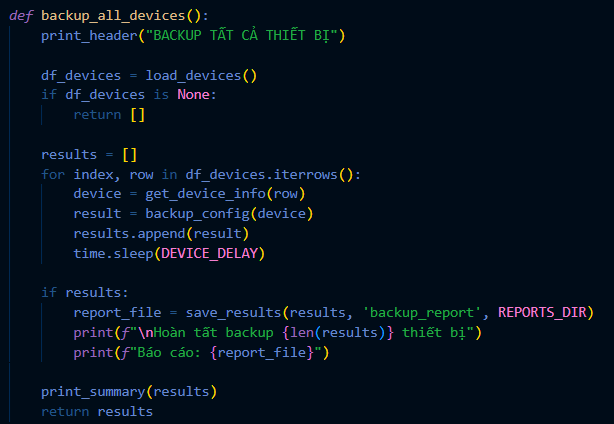
\includegraphics[width=0.7\textwidth]{image/bu_a_cf.png}
                \caption{Cấu hình backup cho tất cả thiết bị}
        \end{figure}
        \item restore\_config():Restore cấu hình từ file backup.
            \begin{figure}[H]
                \centering
                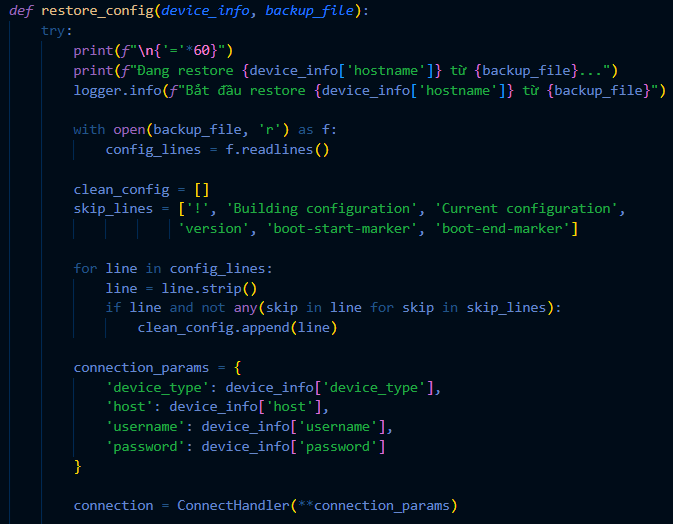
\includegraphics[width=0.7\textwidth]{image/rs_cf_1.png}
            \end{figure}

            \begin{figure}[H]
                \centering
                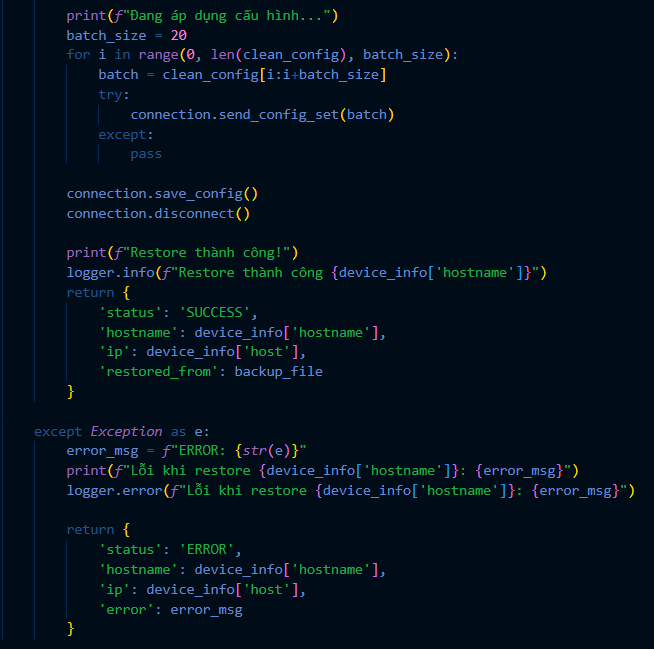
\includegraphics[width=0.7\textwidth]{image/rs_cf_2.png}
                \caption{Cấu hình lưu trữ}
            \end{figure}
            
        \item restore\_device():Cho phép chọn thiết bị và file backup để restore.
        \begin{figure}[H]
                \centering
                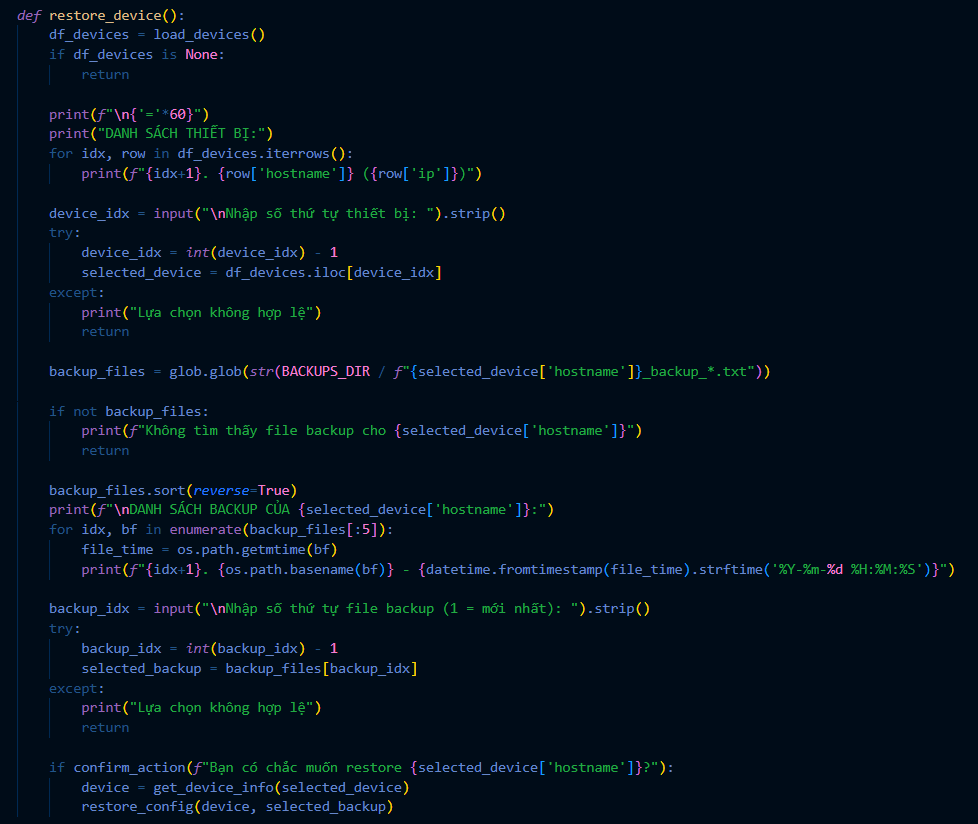
\includegraphics[width=0.7\textwidth]{image/rs_dv.png}
                \caption{Cấu hình lưu trữ thiết bị}
        \end{figure}
        \item simulate\_and\_restore():Mô phỏng lỗi (xóa subinterface) và tự động khôi phục.
        \begin{figure}[H]
                \centering
                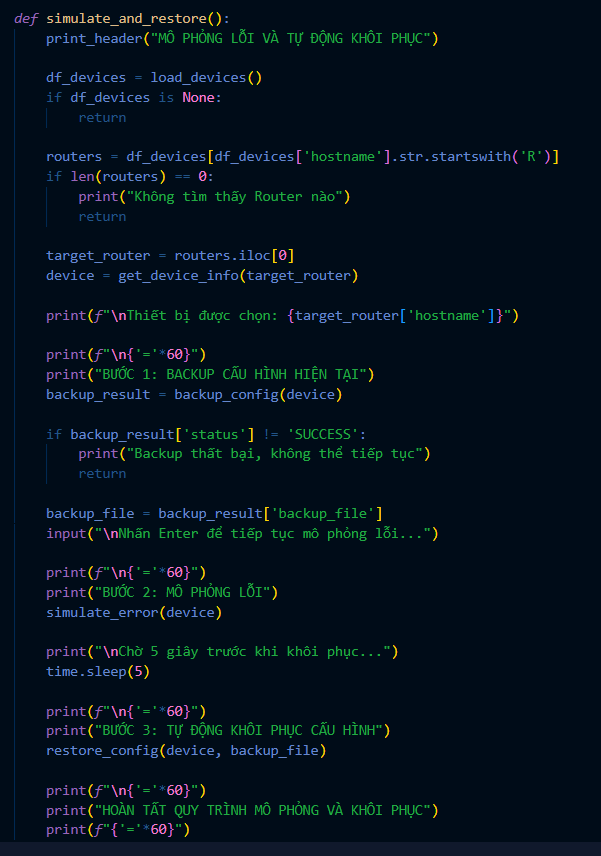
\includegraphics[width=0.7\textwidth]{image/sml_&_rs.png}
                \caption{Cấu hình mô phỏng lỗi và lưu trữ}
        \end{figure}
        \item list\_backups():Hiển thị danh sách các file backup.
        \begin{figure}[H]
                \centering
                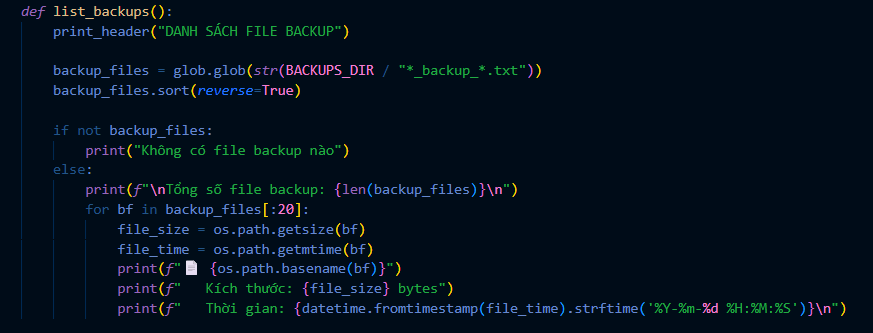
\includegraphics[width=0.7\textwidth]{image/l_bu.png}
                \caption{Cấu hình hiển thị danh sách backup}
        \end{figure}
        \item simulate\_error():Tạo lỗi giả lập bằng cách xóa cấu hình subinterface.
        \begin{figure}[H]
                \centering
                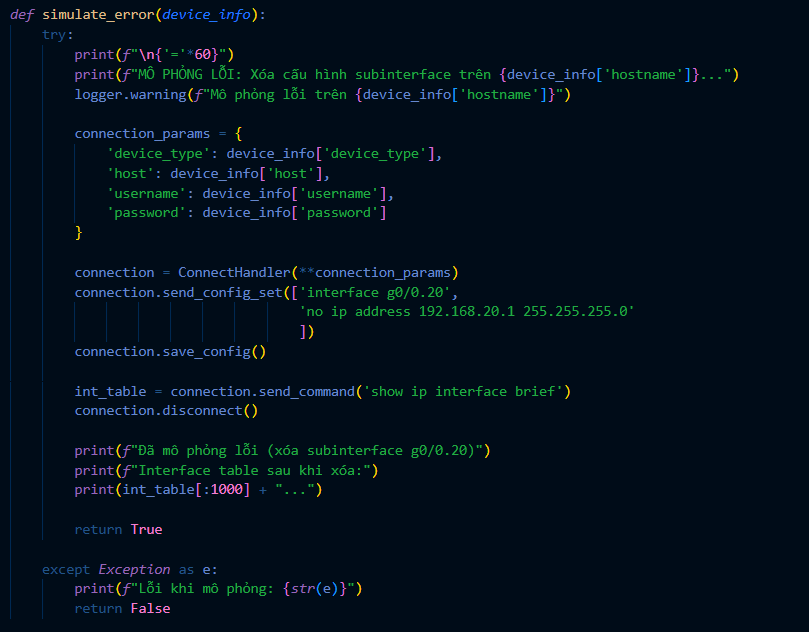
\includegraphics[width=0.7\textwidth]{image/sml_e.png}
                \caption{Cấu hình giả lập lỗi}
        \end{figure}
    \end{itemize}

\subsubsection{monitoring.py - Module giám sát thiết bị}
    Mục đích:Giám sát và kiểm tra trạng thái thiết bị mạng.
    Các hàm chính:
    \begin{itemize}
        \item check\_device\_connectivity(): Kiểm tra kết nối đến các thiết bị, đo response time.
        \begin{figure}[H]
                \centering
                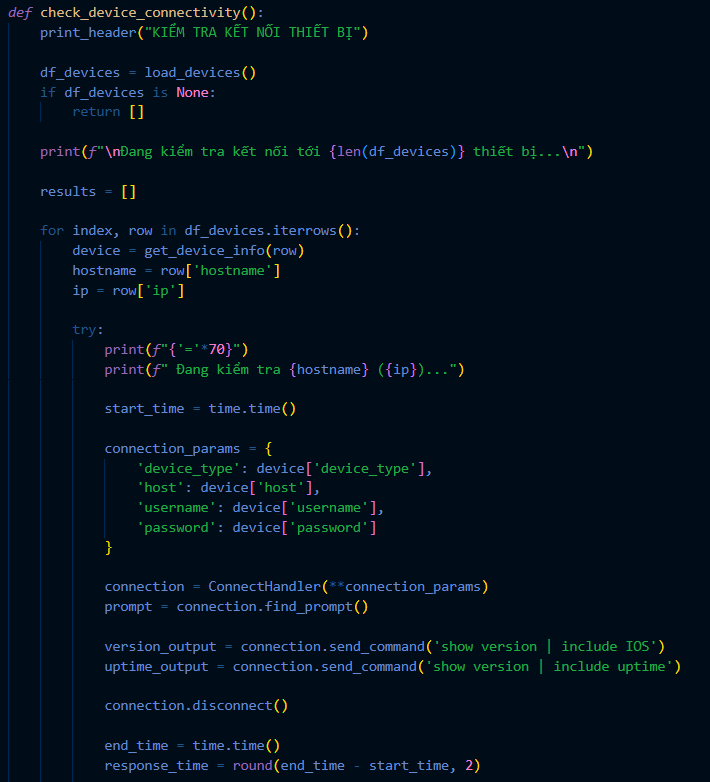
\includegraphics[width=0.7\textwidth]{image/ch_d_co_1.png}
        \end{figure}
        
        \begin{figure}[H]
                \centering
                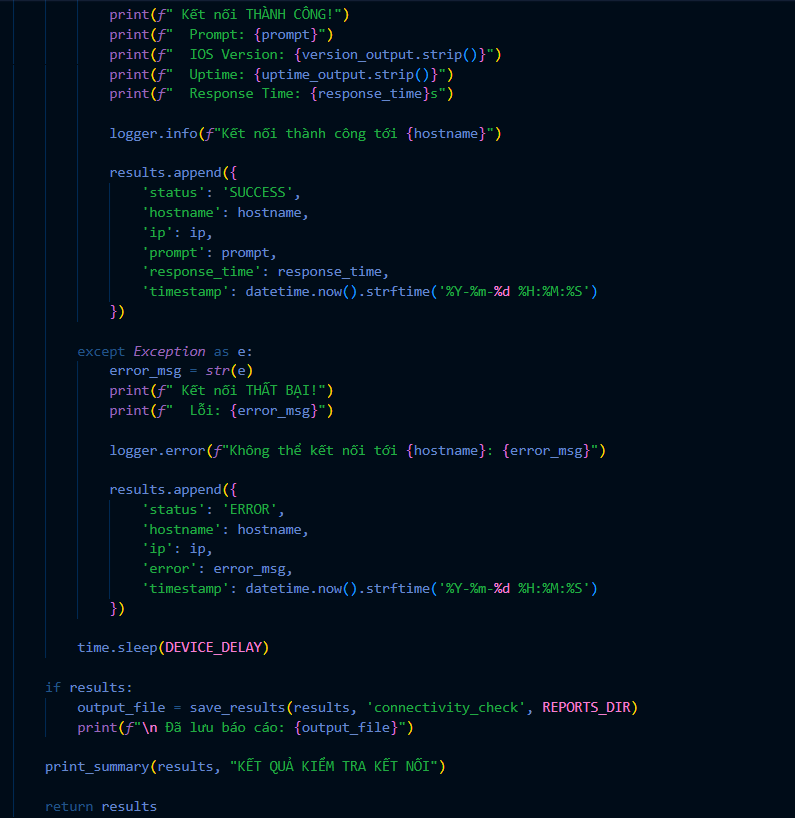
\includegraphics[width=0.7\textwidth]{image/ch_d_co_2.png}
                \caption{Cấu hình kiểm tra kết nối cho các thiết bị}
        \end{figure}
               
        \item show\_interface\_status(): Hiển thị trạng thái interface (up/down).
        \begin{figure}[H]
                \centering
                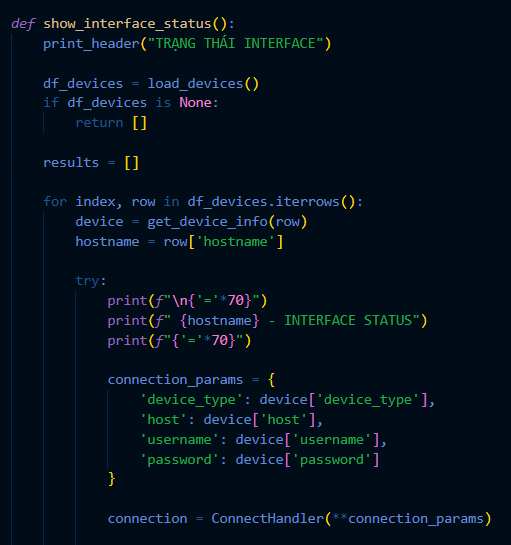
\includegraphics[width=0.7\textwidth]{image/sh_if_ st_1.png}
                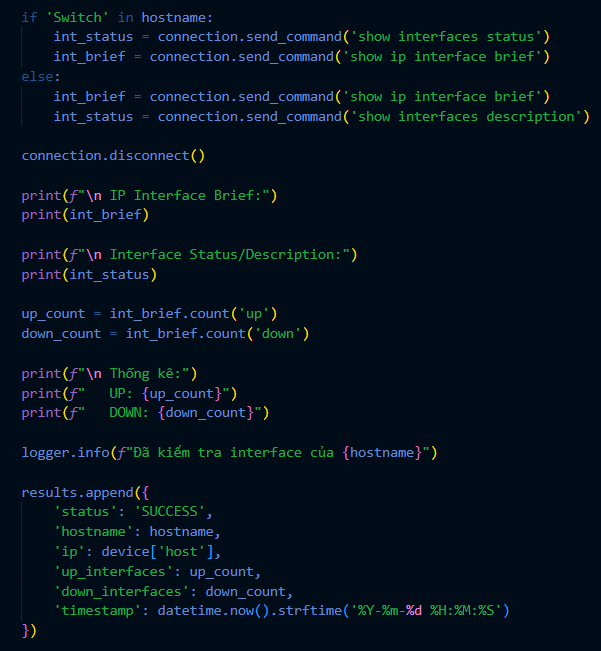
\includegraphics[width=0.7\textwidth]{image/sh_if_st_2.png}
                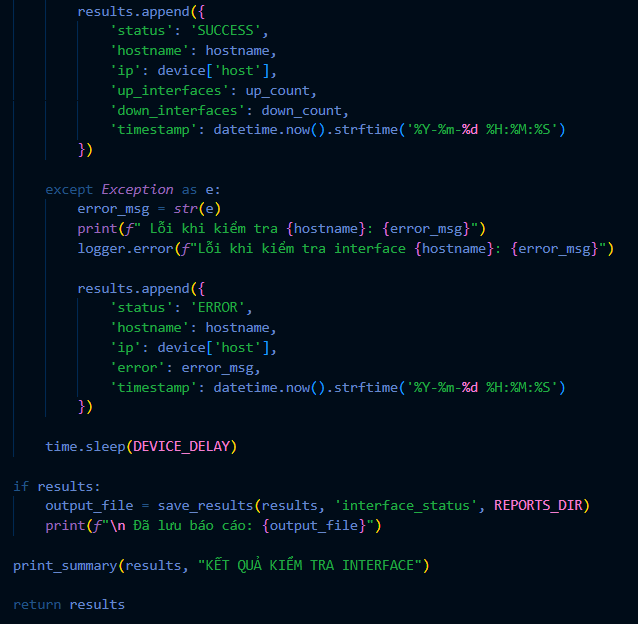
\includegraphics[width=0.7\textwidth]{image/sh_if_st_3.png}
                \caption{Cấu hình hiển thị trạng thái interface}
        \end{figure}
        \item show\_routing\_table(): Xem bảng định tuyến của Router.
        \begin{figure}[H]
                \centering
                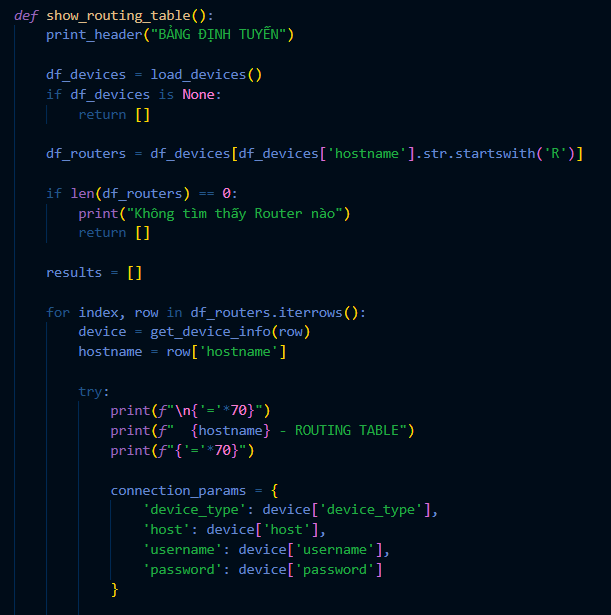
\includegraphics[width=0.7\textwidth]{image/sh_to_tb_1.png}
        \end{figure}

        \begin{figure}[H]
                \centering
                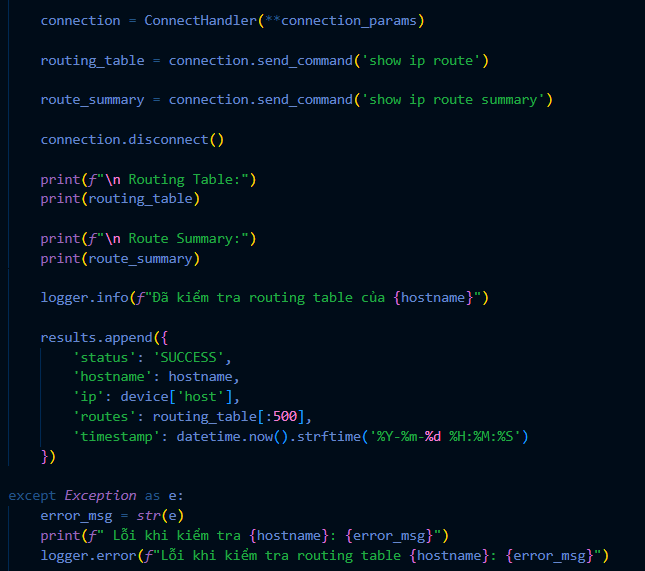
\includegraphics[width=0.7\textwidth]{image/sh_to_tb_2.png}
        \end{figure}

         \begin{figure}[H]
                \centering
                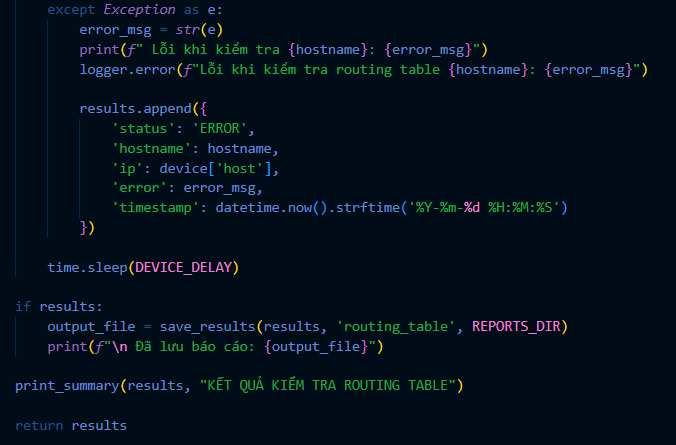
\includegraphics[width=0.7\textwidth]{image/sh_ro_tb_3.png}
                \caption{Cấu hình hiển thị định tuyến của Router}
        \end{figure}

        
        \item show\_vlan\_info(): Xem thông tin VLAN trên Switch.
        \begin{figure}[H]
                \centering
                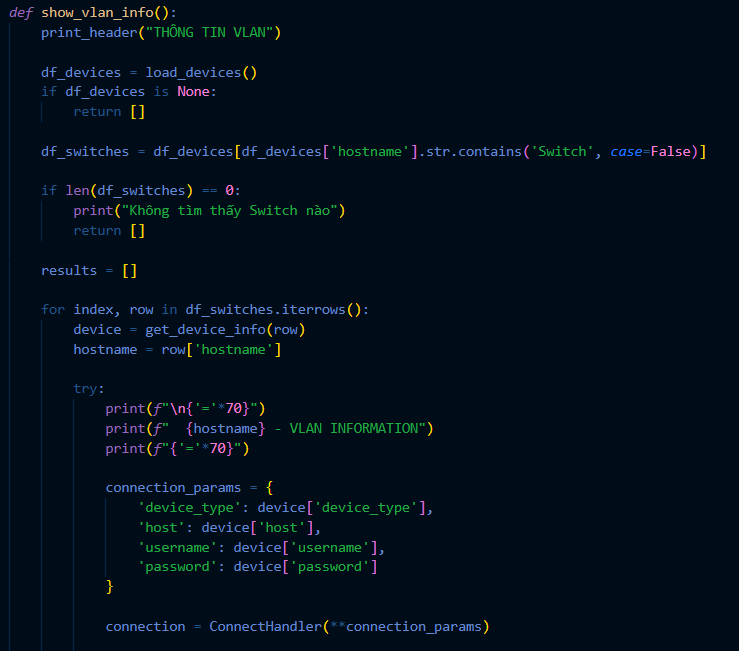
\includegraphics[width=0.7\textwidth]{image/sh_vl_i_1.png}
                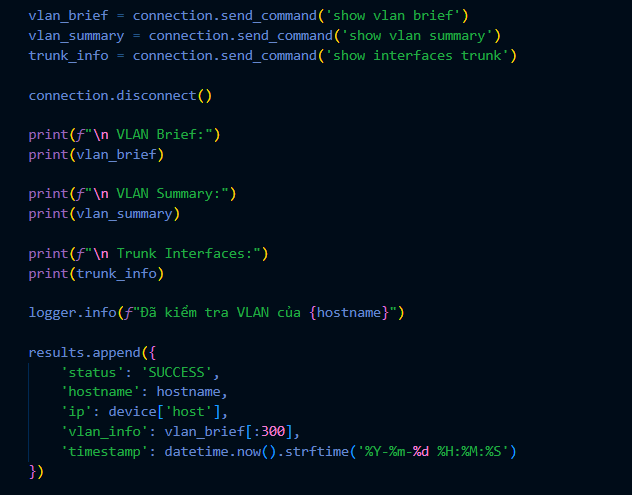
\includegraphics[width=0.7\textwidth]{image/sh_vl_i_2.png}
        \end{figure}

        \begin{figure}[H]
                \centering
                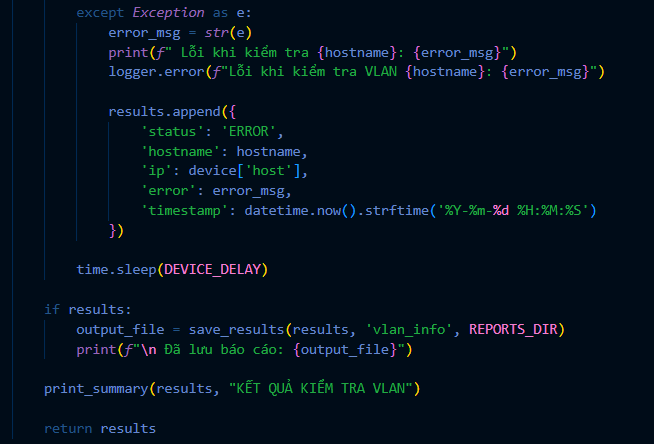
\includegraphics[width=0.7\textwidth]{image/sh_vl_i_3.png}
                \caption{Cấu hình hiển thị VLAN trên Switch}
        \end{figure}
        
        \item show\_ospf\_status(): Xem trạng thái OSPF (neighbors, database).
        \begin{figure}[H]
                \centering
                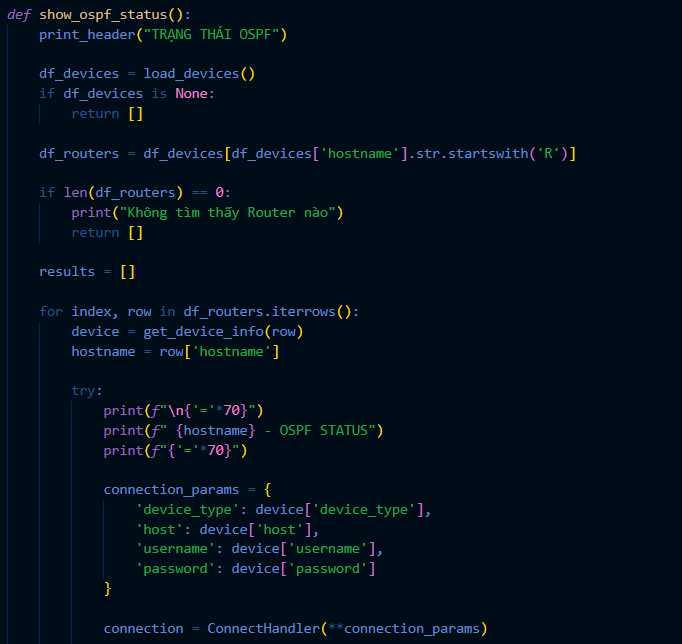
\includegraphics[width=0.7\textwidth]{image/sh_ospf_st_1.png}
        \end{figure}

        \begin{figure}[H]
                \centering
                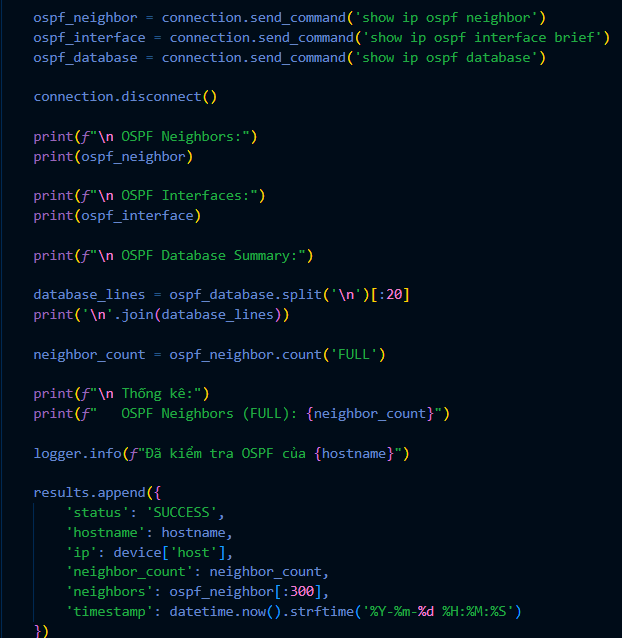
\includegraphics[width=0.7\textwidth]{image/sh_ospf_st_2.png}
        \end{figure}

        \begin{figure}[H]
                \centering
                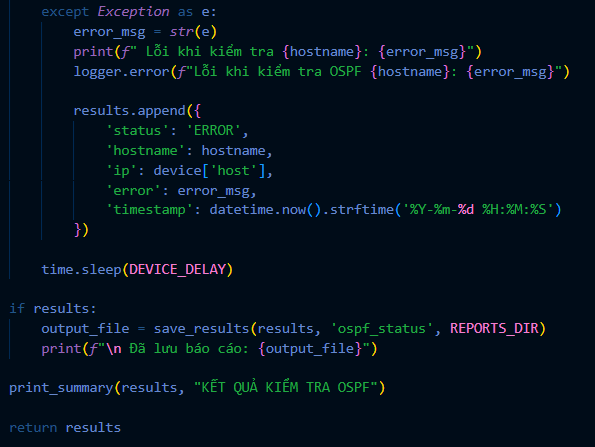
\includegraphics[width=0.7\textwidth]{image/sh_ospf_st_3.png}
                \caption{Cấu hình hiển thị trạng thái OSPF}
        \end{figure}
        
        \item monitor\_all\_devices(): Giám sát toàn diện (chạy tất cả các kiểm tra trên).
        \begin{figure}[H]
                \centering
                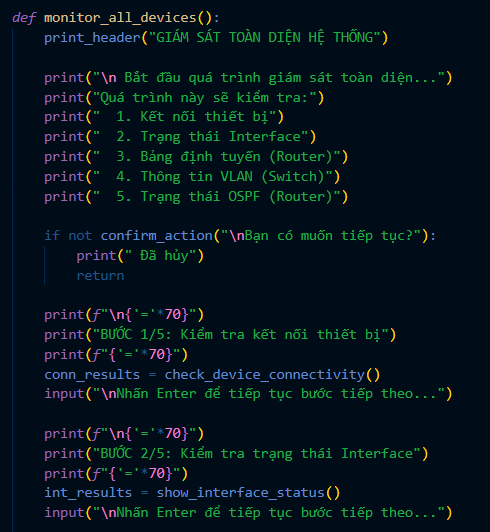
\includegraphics[width=0.7\textwidth]{image/mn_a_d_1.png}
        \end{figure}

        \begin{figure}[H]
                \centering
                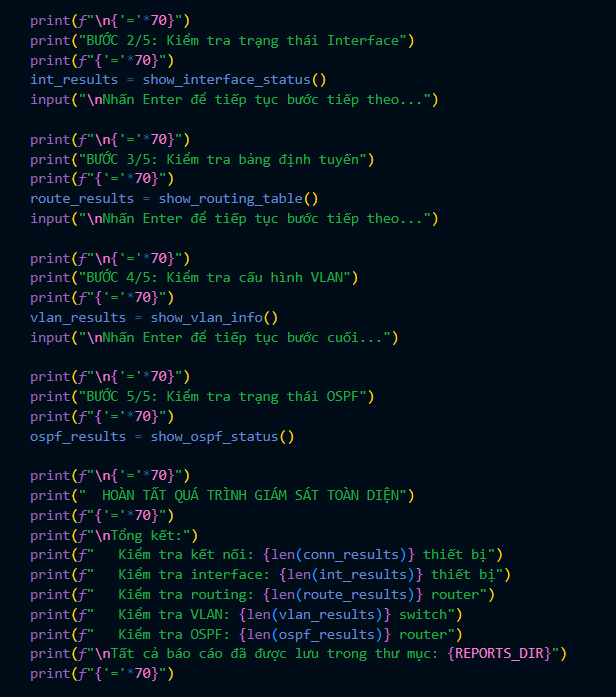
\includegraphics[width=0.7\textwidth]{image/mn_a_d_2.png}
                \caption{Cấu hình định giám sát toàn diện}
        \end{figure}
        
        \item monitoring\_menu(): Menu cho các chức năng giám sát.
        \begin{figure}[H]
                \centering
                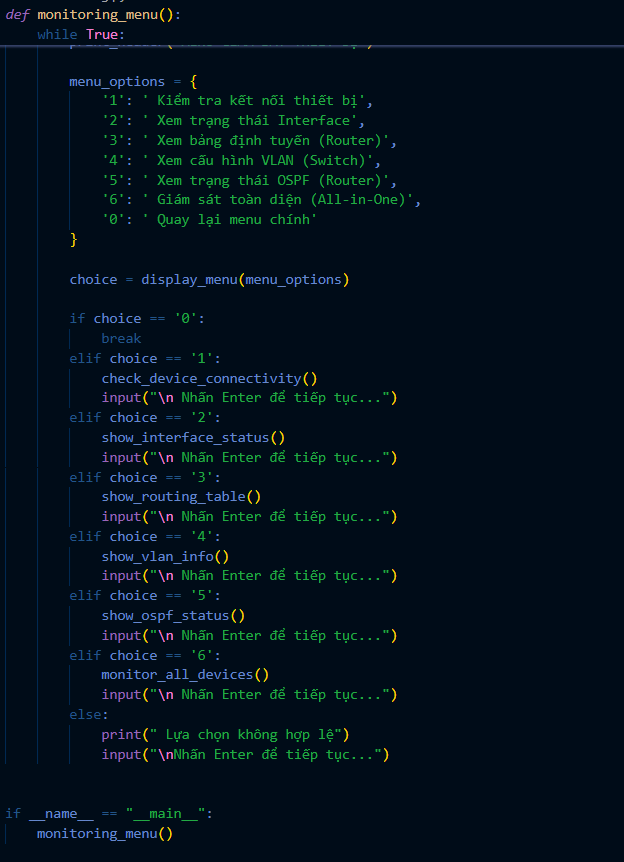
\includegraphics[width=0.7\textwidth]{image/mn_menu.png}
                \caption{Danh sách của các chức năng giám sát}
        \end{figure}
    \end{itemize}

\subsubsection{main.py - File chính của chương trình}
    Mục đích:Chạy toàn bộ các module, cung cấp giao diện menu cho người dung
    Các chức năng chính:
    \begin{itemize}
        \item show\_welcome():Hiển thị màn hình chào mừng.
        
        \begin{figure}[H]
                \centering
                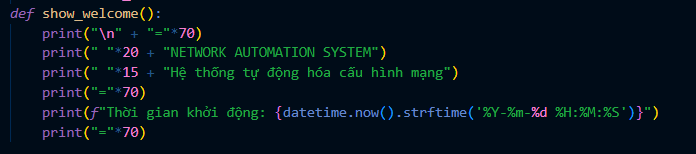
\includegraphics[width=0.7\textwidth]{image/sh_welcome.png}
                \caption{Cấu hình hiển thị chào mừng}
        \end{figure}
        
        \item configuration\_menu():Menu cấu hình thiết bị (VLAN, IP, OSPF, Static Route).
        
        \begin{figure}[H]
                \centering
                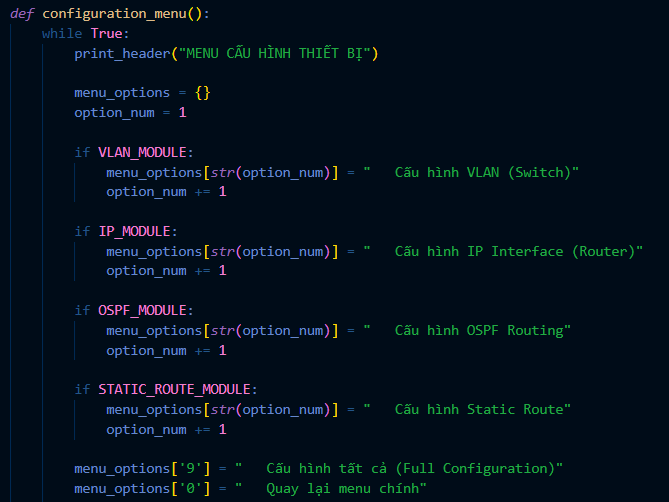
\includegraphics[width=0.7\textwidth]{image/cf_menu_1.png}
        \end{figure}

        \begin{figure}[H]
                \centering
                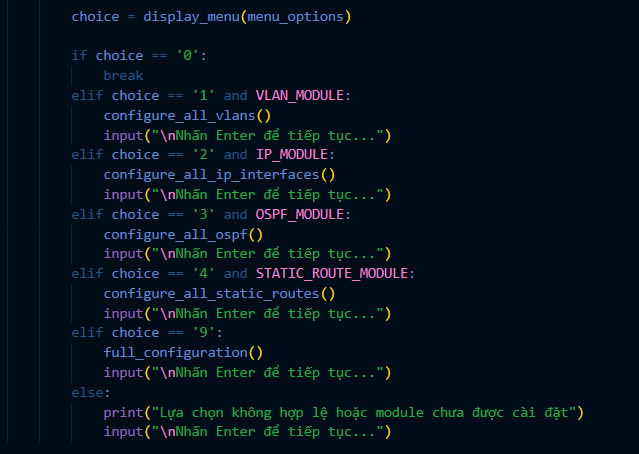
\includegraphics[width=0.7\textwidth]{image/cf_menu_2.png}
                \caption{Cấu hình hiển thị danh sách}
        \end{figure}
          
        \item backup\_restore\_menu():Menu backup và restore cấu hình.
        
        \begin{figure}[H]
                \centering
                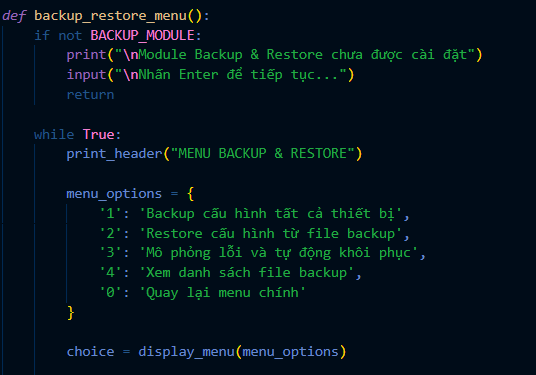
\includegraphics[width=0.7\textwidth]{image/bu_rs_menu_1.png}
        \end{figure}
        
        \begin{figure}[H]
                \centering
                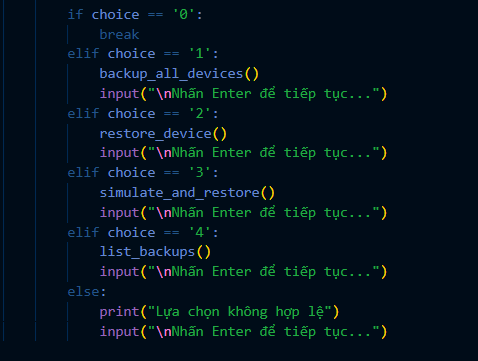
\includegraphics[width=0.7\textwidth]{image/bu_rs_menu_2.png}
                \caption{Cấu hình danh sách lưu trữ và sao lưu}
        \end{figure}
        
        \item monitoring\_menu():Menu giám sát thiết bị.
        
         \begin{figure}[H]
                \centering
                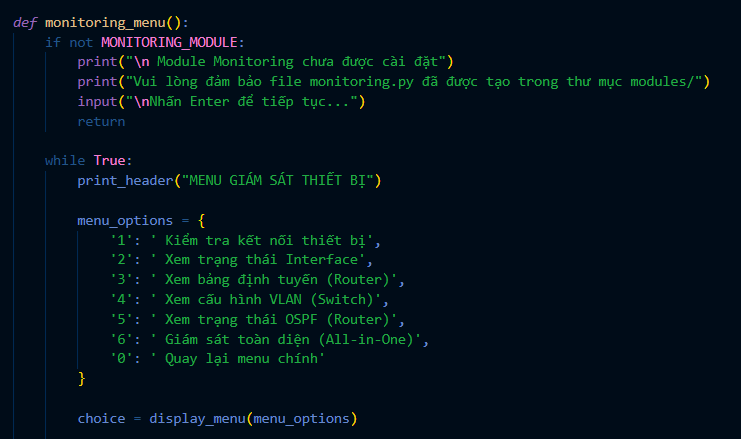
\includegraphics[width=0.7\textwidth]{image/mn_menu_1.png}
        \end{figure}

        \begin{figure}[H]
                \centering
                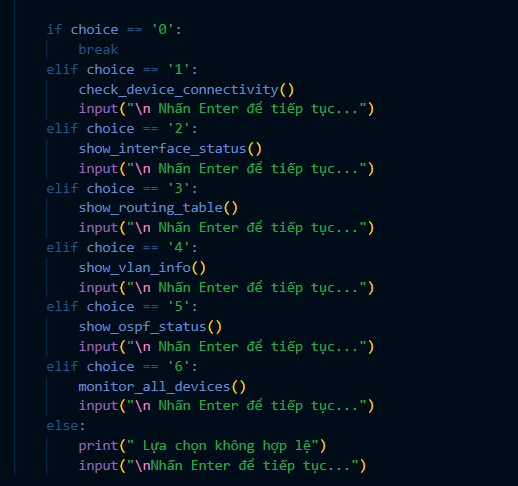
\includegraphics[width=0.7\textwidth]{image/mn_menu_2.png}
                \caption{Cấu hình danh sách giám sát thiết bị}
        \end{figure}
        
        \item full\_configuration():Thực hiện cấu hình đầy đủ toàn bộ hệ thống theo 4 bước.

        \begin{figure}[H]
                \centering
                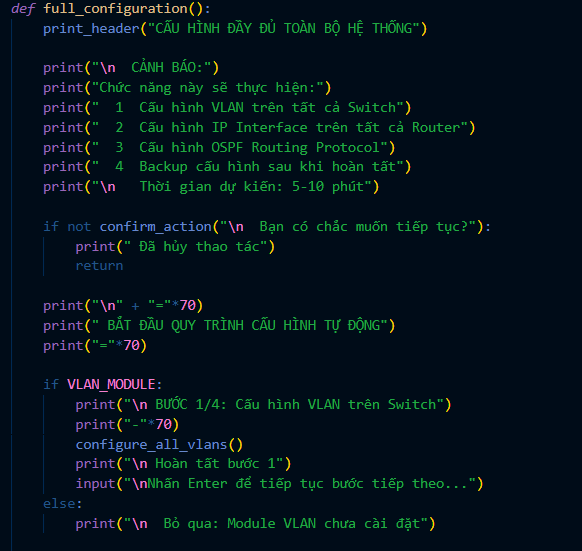
\includegraphics[width=0.7\textwidth]{image/full_cf_1.png}
                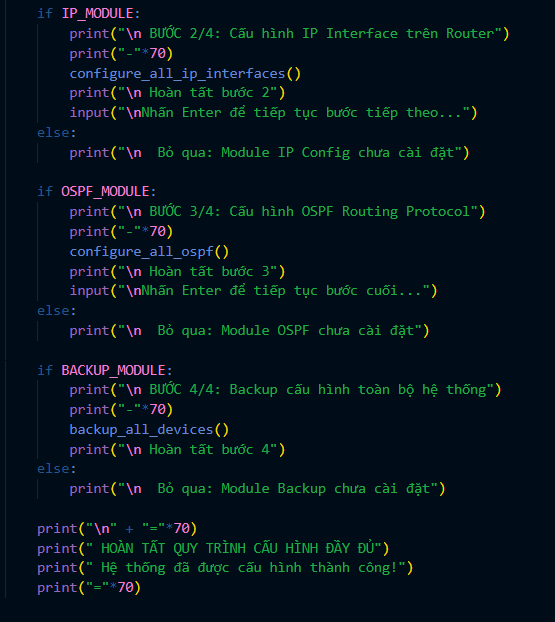
\includegraphics[width=0.7\textwidth]{image/full_cf_2.png}
                \caption{Cấu hình toàn bộ hệ thống}
        \end{figure}
        
        \item system\_info():Hiển thị thông tin hệ thống, modules đã cài đặt.

        \begin{figure}[H]
                \centering
                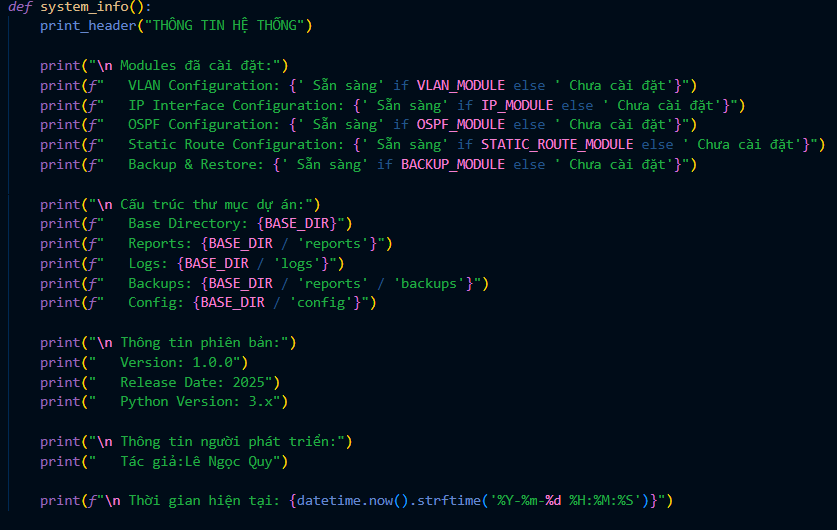
\includegraphics[width=0.7\textwidth]{image/sys_i4.png}
                \caption{Cấu hình hiển thị thông tin hệ thống}
        \end{figure}
        
        \item main\_menu():Menu chính với 4 lựa chọn chính.

        \begin{figure}[H]
                \centering
                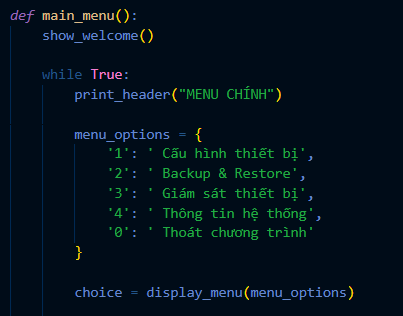
\includegraphics[width=0.7\textwidth]{image/main_menu_1.png}
        \end{figure}

        \begin{figure}[H]
                \centering
                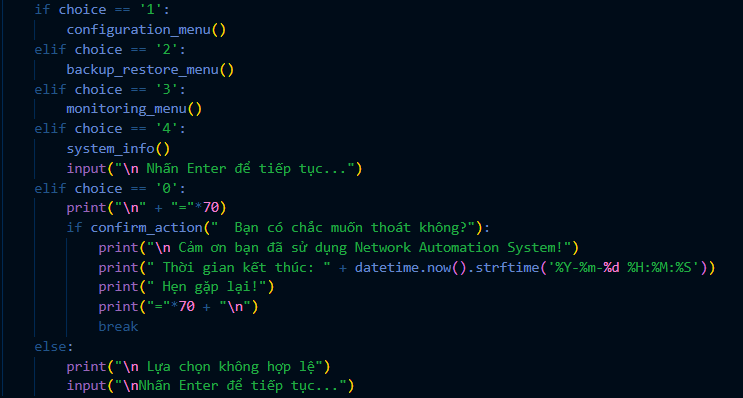
\includegraphics[width=0.7\textwidth]{image/main_menu_2.png}
                \caption{Cấu hình hiển thị thông tin hệ thống}
        \end{figure}

        
        \item main():Hàm khởi chạy chương trình, xử lý ngoại lệ.

        \begin{figure}[H]
                \centering
                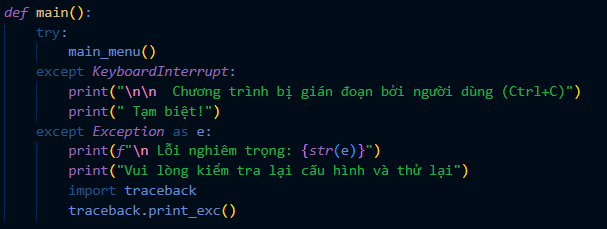
\includegraphics[width=0.7\textwidth]{image/main.png}
                \caption{Cấu hình hiển thị thông tin hệ thống}
        \end{figure}
        
    \end{itemize}

\subsection{Quy trình cấu hình đầy đủ}
\subsubsection{Phần 1: Cấu hình VLAN (vlan_config.py)}
        \begin{itemize}
            \item Đọc danh sách thiết bị và lọc Switch.
            \begin{figure}[H]
                \centering
                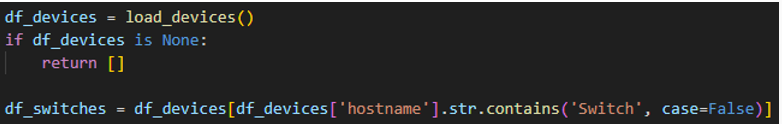
\includegraphics[width=0.7\textwidth]{image/1.png}
            \end{figure}
            Kết quả: Switch1, Switch2, Switch3

            \item Lặp qua từng Switch
            \begin{figure}[H]
                \centering
                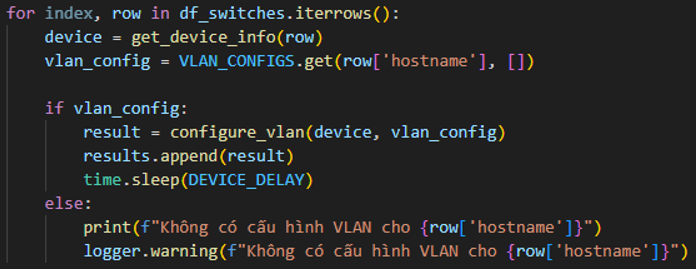
\includegraphics[width=0.7\textwidth]{image/2.png}
            \end{figure}

            \item Kết nối đến Switch
            \begin{figure}[H]
                \centering
                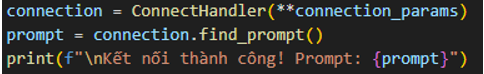
\includegraphics[width=0.7\textwidth]{image/3.png}
            \end{figure}
            \item Gửi lệnh cấu hình VLAN
            \begin{figure}[H]
                \centering
                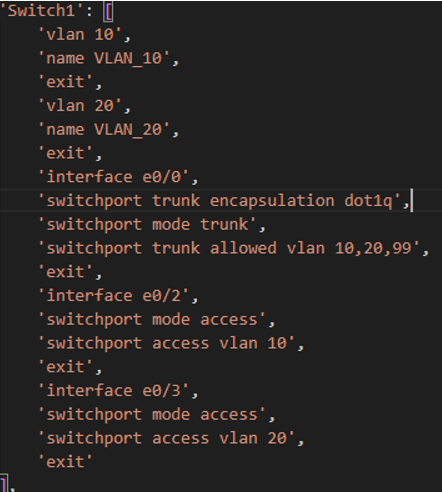
\includegraphics[width=0.7\textwidth]{image/gui_cau_hinh_vlan.png}
            \end{figure}

            \begin{figure}[H]
                \centering
                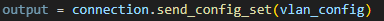
\includegraphics[width=0.7\textwidth]{image/4.png}
            \end{figure}

            \item Lưu cấu hình\\
            connection.save\_config()\\
            Thực hiện: write memory hoặc copy run start
            \item Kiểm tra kết quả \\
            verify\_output = connection.send\_command('show vlan brief')
            \item  Ngắt kết nối\\
            connection.disconnect()
            \item Lưu kết quả \\
            \begin{figure}[H]
                \centering
                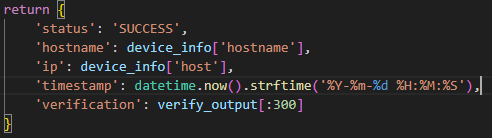
\includegraphics[width=0.7\textwidth]{image/5.png}
            \end{figure}
            \item Lặp lại cho Switch2, Switch3 \\
            time.sleep(DEVICE\_DELAY)  \\
            Tiếp tục với Switch2, Switch3
            \item Xuất báo cáo \\
            output\_file = save\_results(results, 'vlan\_config\_results', REPORTS\_DIR)\\
            File: reports/vlan\_config\_results\_20250122\_103055.csv\\
            Nội dung CSV:
            \begin{figure}[H]
                \centering
                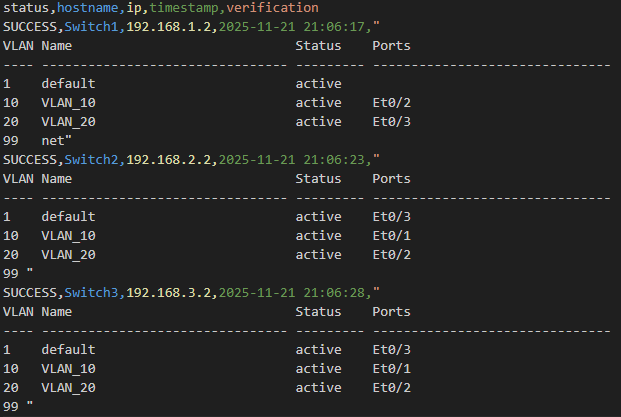
\includegraphics[width=0.7\textwidth]{image/6.png}
            \end{figure}
        \end{itemize}
\subsubsection{Phần 2: Cấu hình IP interface (ip/_config.py)}
        \begin{itemize}
            \item Đọc danh sách thiết bị và lọc Router
            \begin{figure}[H]
                \centering
                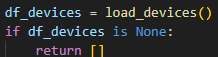
\includegraphics[width=0.7\textwidth]{image/7.png}
            \end{figure}
            Không lọc, lấy tất cả thiết bị (R1, R2, R3 có IP\_CONFIGS)
            \item Kết nối đến R1
            \begin{figure}[H]
                \centering
                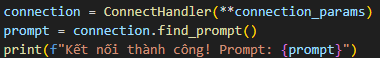
\includegraphics[width=0.7\textwidth]{image/8.png}
            \end{figure}
            \item Gửi lệnh cấu hình IP
            \begin{figure}[H]
                \centering
                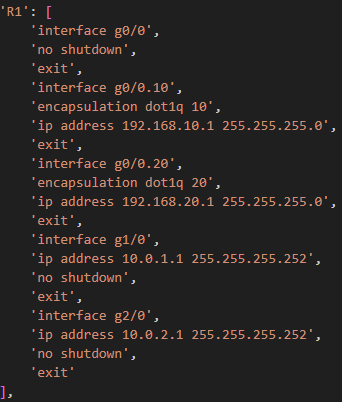
\includegraphics[width=0.7\textwidth]{image/9.png}
            \end{figure}
            \begin{figure}[H]
                \centering
                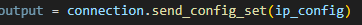
\includegraphics[width=0.7\textwidth]{image/10.png}
            \end{figure}
            \item Lưu và verify
            \begin{figure}[H]
                \centering
                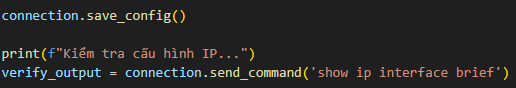
\includegraphics[width=0.7\textwidth]{image/11.png}
            \end{figure}
            Output:
            \begin{figure}[H]
                \centering
                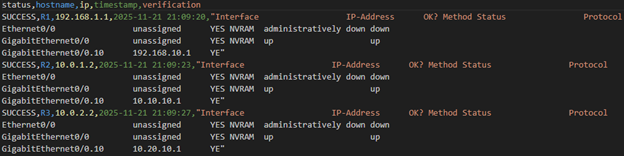
\includegraphics[width=0.7\textwidth]{image/12.png}
            \end{figure}
            \item Lặp lại cho R2, R3
        \end{itemize}    
\subsubsection{Phần 3: Cấu hình OSPF (ospf_config.py)}
        \begin{itemize}
            \item Đọc danh sách thiết bị và lọc Router
            \begin{figure}[H]
                \centering
                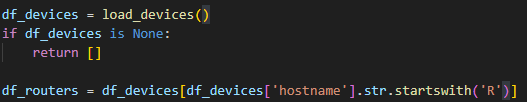
\includegraphics[width=0.7\textwidth]{image/13.png}
            \end{figure}
             Kết quả: R1, R2, R3
             \item Cấu hình OSPF cho R1
             \begin{figure}[H]
                \centering
                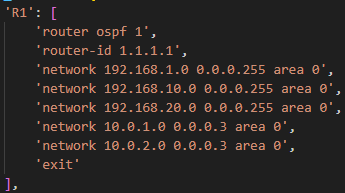
\includegraphics[width=0.7\textwidth]{image/14.png}
            \end{figure}
            \begin{figure}[H]
                \centering
                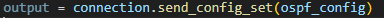
\includegraphics[width=0.7\textwidth]{image/15.png}
            \end{figure}
            \item Chờ OSPF neighbor thiết lập
            \begin{figure}[H]
                \centering
                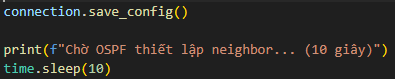
\includegraphics[width=0.7\textwidth]{image/16.png}
            \end{figure}
            \item Verify OSPF
            \begin{figure}[H]
                \centering
                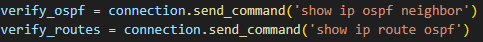
\includegraphics[width=0.7\textwidth]{image/17.png}
            \end{figure}
            Output:
            \begin{figure}[H]
                \centering
                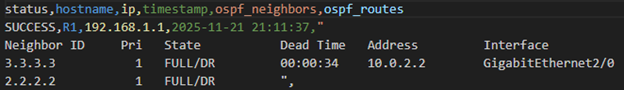
\includegraphics[width=0.7\textwidth]{image/18.png}
            \end{figure}
             Lặp lại cho R2, R3
        \end{itemize}    
\subsubsection{Phần 4: Backup cấu hình (backup_restore.py)} 
        \begin{itemize}
            \item Backup tất cả thiết bị
            \begin{figure}[H]
                \centering
                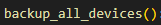
\includegraphics[width=0.7\textwidth]{image/19.png}
            \end{figure}
            \item Lặp qua từng thiết bị
            \begin{figure}[H]
                \centering
                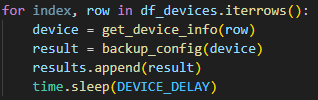
\includegraphics[width=0.7\textwidth]{image/20.png}
            \end{figure}
            \item Kết nối và lấy running-config
            \begin{figure}[H]
                \centering
                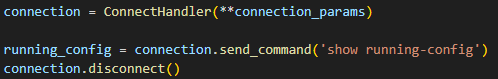
\includegraphics[width=0.7\textwidth]{image/21.png}
            \end{figure}
            Nội dung running\_config:
            \begin{figure}[H]
                \centering
                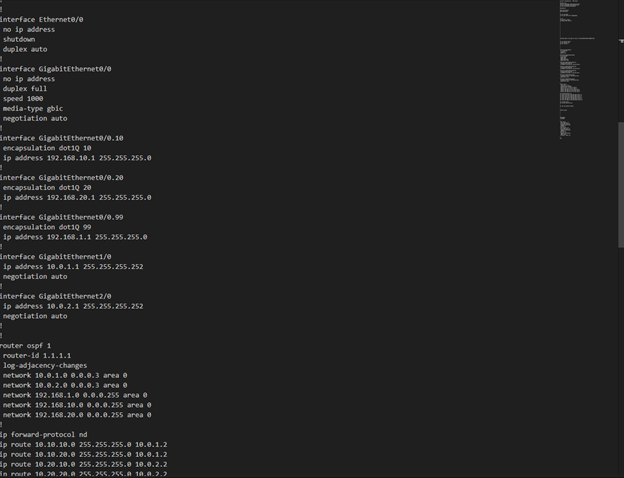
\includegraphics[width=0.7\textwidth]{image/22.png}
            \end{figure}
            \item Lưu vào file
            \begin{figure}[H]
                \centering
                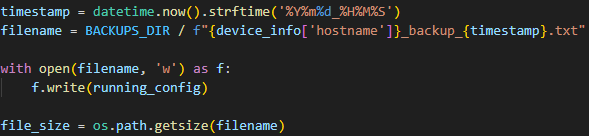
\includegraphics[width=0.7\textwidth]{image/23.png}
            \end{figure}
            \item Kết quả backup
            \begin{figure}[H]
                \centering
                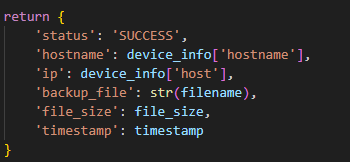
\includegraphics[width=0.7\textwidth]{image/24.png}
            \end{figure}
            \item Lặp lại cho tất cả thiết bị
            Kết quả:
            \begin{verbatim}
                R1_backup_20251122_104500.txt
                R2_backup_20251122_104505.txt
                R3_backup_20251122_104510.txt
                Switch1_backup_20251122_104515.txt
                Switch2_backup_20251122_104520.txt
                Switch3_backup_20251122_104525.txt
            \end{verbatim}
            \item  Xuất báo cáo backup
            \begin{figure}[H]
                \centering
                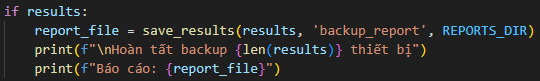
\includegraphics[width=0.7\textwidth]{image/25.png}
            \end{figure}
        \end{itemize}
\subsubsection{Phần 3: Quy trình giám sát (monitoring.py)}    
CHỨC NĂNG 1: Kiểm tra kết nối (check\_device\_connectivity)
    \begin{itemize}
        \item Lặp qua từng thiết bị
        \begin{figure}[H]
            \centering
            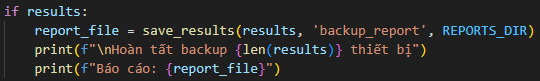
\includegraphics[width=0.7\textwidth]{image/26.png}
        \end{figure}
        \item Kết nối và đo thời gian
        \begin{figure}[H]
            \centering
            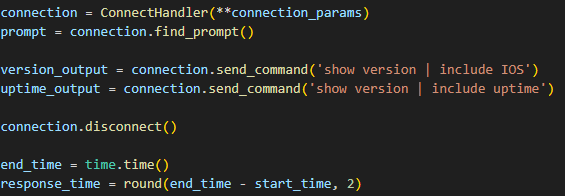
\includegraphics[width=0.7\textwidth]{image/27.png}
        \end{figure}
        \item  Lưu kết quả
        \begin{figure}[H]
            \centering
            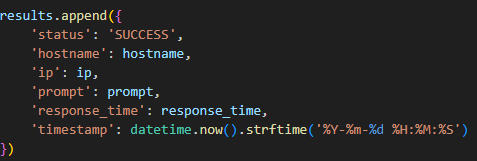
\includegraphics[width=0.7\textwidth]{image/28.png}
        \end{figure}
    \end{itemize}
CHỨC NĂNG 2: Xem trạng thái Interface (show\_interface\_status)       
    \begin{itemize}
        \item Với Switch
        \begin{figure}[H]
            \centering
            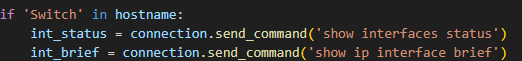
\includegraphics[width=0.7\textwidth]{image/29.png}
        \end{figure}
        \item  Với Router
        \begin{figure}[H]
            \centering
            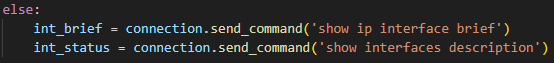
\includegraphics[width=0.7\textwidth]{image/30.png}
        \end{figure}
        \item Thống kê
        \begin{figure}[H]
            \centering
            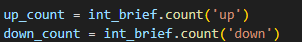
\includegraphics[width=0.7\textwidth]{image/31.png}
        \end{figure}
    \end{itemize}
CHỨC NĂNG 3: Xem bảng định tuyến (show\_routing\_table)
    \begin{itemize}
        \item Chỉ áp dụng cho Router
        \begin{figure}[H]
            \centering
            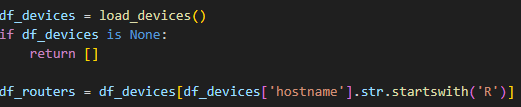
\includegraphics[width=0.7\textwidth]{image/32.png}
        \end{figure}
        \item  Lấy routing table
        \begin{figure}[H]
            \centering
            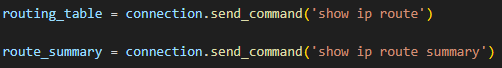
\includegraphics[width=0.7\textwidth]{image/33.png}
        \end{figure}
    \end{itemize}
CHỨC NĂNG 4: Xem VLAN (show\_vlan\_info)
    \begin{itemize}
        \item Chỉ áp dụng cho Switch
         \begin{figure}[H]
            \centering
            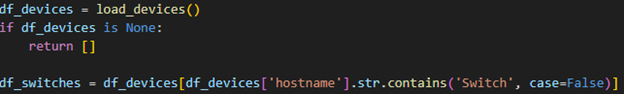
\includegraphics[width=0.7\textwidth]{image/34.png}
        \end{figure}
        \item Lấy thông tin VLAN
        \begin{figure}[H]
            \centering
            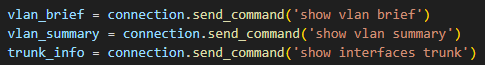
\includegraphics[width=0.7\textwidth]{image/35.png}
        \end{figure}
    \end{itemize}
CHỨC NĂNG 5: Xem OSPF Status (show\_ospf\_status)
    \begin{itemize}
        \item Lấy thông tin OSPF
        \begin{figure}[H]
            \centering
            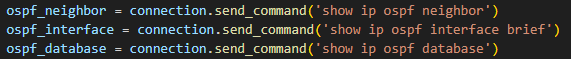
\includegraphics[width=0.7\textwidth]{image/36.png}
        \end{figure}
        \item  Đếm số neighbor 
        \begin{figure}[H]
            \centering
            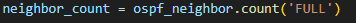
\includegraphics[width=0.7\textwidth]{image/37.png}
        \end{figure}
    \end{itemize}
CHỨC NĂNG 6: Giám sát toàn diện (monitor\_all\_devices)            
    \begin{itemize}
        \item Quy trình:
             \begin{verbatim}
                1.Kiểm tra kết nối → Báo cáo CSV
                2.Kiểm tra Interface → Báo cáo CSV
                3.Kiểm tra Routing Table → Báo cáo CSV
                4.Kiểm tra VLAN → Báo cáo CSV
                5.Kiểm tra OSPF → Báo cáo CSV
                Kết quả: 5 file báo cáo trong thư mục reports/
            \end{verbatim}    
    \end{itemize}
\subsubsection{Phần 4: Quy trình backup/restore}
TÍNH NĂNG 1: Restore từ file backup
    \begin{itemize}
        \item  Chọn thiết bị cần restore
        \begin{figure}[H]
            \centering
            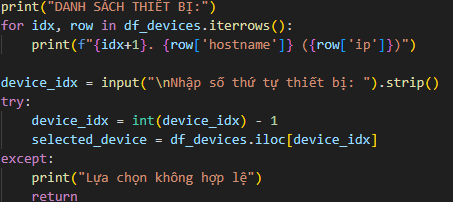
\includegraphics[width=0.7\textwidth]{image/38.png}
        \end{figure}
        \item Hiển thị các file backup
        \begin{figure}[H]
            \centering
            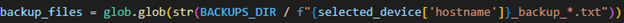
\includegraphics[width=0.7\textwidth]{image/39.png}
        \end{figure}
        \item Chọn file backup
        \begin{figure}[H]
            \centering
            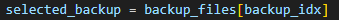
\includegraphics[width=0.7\textwidth]{image/40.png}
        \end{figure}
        \item Xác nhận restore
        \begin{figure}[H]
            \centering
            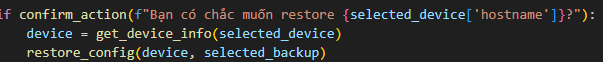
\includegraphics[width=0.7\textwidth]{image/41.png}
        \end{figure}
        \item Đọc file backup
        \begin{figure}[H]
            \centering
            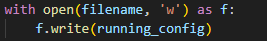
\includegraphics[width=0.7\textwidth]{image/42.png}
        \end{figure}
        \item  Làm sạch cấu hình
        \begin{figure}[H]
            \centering
            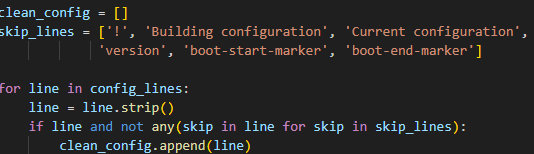
\includegraphics[width=0.7\textwidth]{image/43.png}
        \end{figure}
        \item Áp dụng cấu hình theo batch
        \begin{figure}[H]
            \centering
            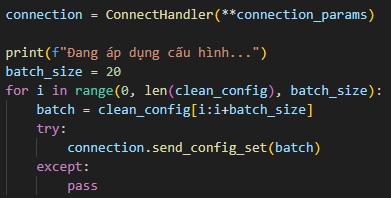
\includegraphics[width=0.7\textwidth]{image/44.png}
        \end{figure}
        \item  Lý do chia batch:
        \begin{verbatim}
            Tránh timeout khi cấu hình quá dài
            Nếu 1 batch lỗi, các batch khác vẫn được áp dụng
            Netmiko có giới hạn số lệnh gửi cùng lúc
        \end{verbatim}
        \item Lưu cấu hình
        \begin{figure}[H]
            \centering
            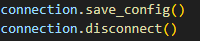
\includegraphics[width=0.7\textwidth]{image/45.png}
        \end{figure}
        \item Kết quả restore
        \begin{figure}[H]
            \centering
            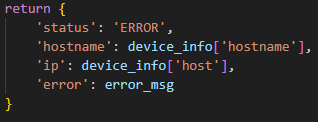
\includegraphics[width=0.7\textwidth]{image/46.png}
        \end{figure}
    \end{itemize}
TÍNH NĂNG 2: Mô phỏng lỗi và tự động khôi phục (simulate\_and\_restore)
    \begin{itemize}
        \item Chọn thiết bị mô phỏng
        \begin{figure}[H]
            \centering
            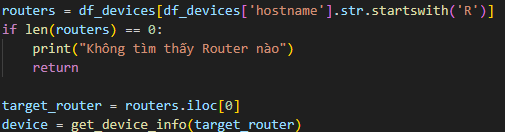
\includegraphics[width=0.7\textwidth]{image/47.png}
        \end{figure}
        \item BƯỚC 1: BACKUP CẤU HÌNH HIỆN TẠI
        \begin{figure}[H]
            \centering
            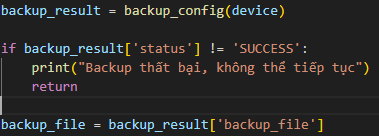
\includegraphics[width=0.7\textwidth]{image/48.png}
        \end{figure}
        \item BƯỚC 2: MÔ PHỎNG LỖI
        \begin{figure}[H]
            \centering
            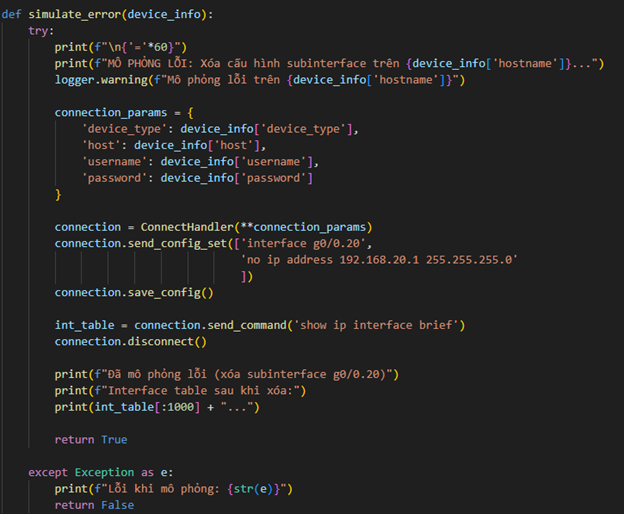
\includegraphics[width=0.7\textwidth]{image/49.png}
        \end{figure}
        \item BƯỚC 3: TỰ ĐỘNG KHÔI PHỤC CẤU HÌNH
        \begin{figure}[H]
            \centering
            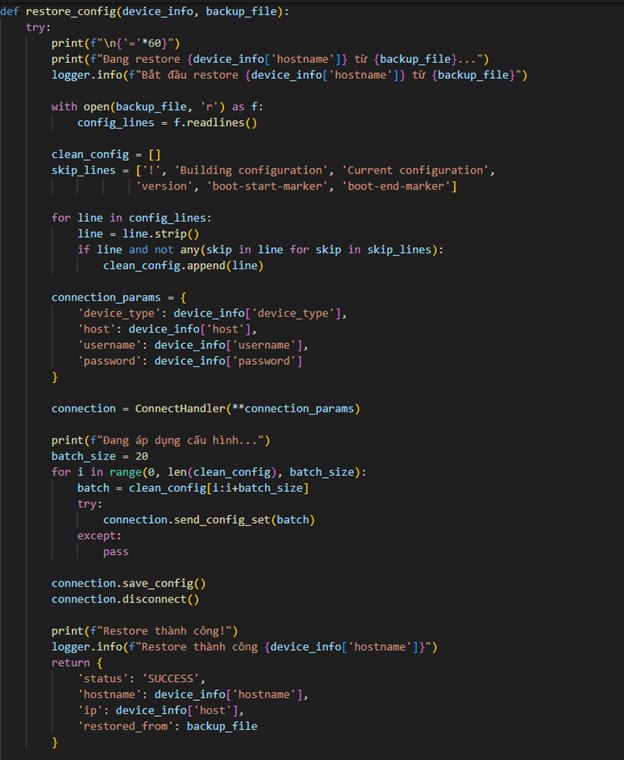
\includegraphics[width=0.7\textwidth]{image/50.png}
        \end{figure}
    \end{itemize}

        



